\documentclass[review]{elsarticle}

\usepackage{lineno,hyperref}
\modulolinenumbers[5]

\journal{Eugène Syriani, University of Montreal}

%%%%%%%%%%%%%%%%%%%%%%%
%% Elsevier bibliography styles
%%%%%%%%%%%%%%%%%%%%%%%
%% To change the style, put a % in front of the second line of the current style and
%% remove the % from the second line of the style you would like to use.
%%%%%%%%%%%%%%%%%%%%%%%

%% Numbered
%\bibliographystyle{model1-num-names}

%% Numbered without titles
%\bibliographystyle{model1a-num-names}

%% Harvard
%\bibliographystyle{model2-names.bst}\biboptions{authoryear}

%% Vancouver numbered
%\usepackage{numcompress}\bibliographystyle{model3-num-names}

%% Vancouver name/year
%\usepackage{numcompress}\bibliographystyle{model4-names}\biboptions{authoryear}

%% APA style
%\bibliographystyle{model5-names}\biboptions{authoryear}

%% AMA style
%\usepackage{numcompress}\bibliographystyle{model6-num-names}

%% `Elsevier LaTeX' style
\bibliographystyle{elsarticle-num}
%%%%%%%%%%%%%%%%%%%%%%%

\begin{document}

\begin{frontmatter}

\title{Visual Parametric Maze Generator DSL \tnoteref{mytitlenote}}
\tnotetext[mytitlenote]{Full source code is available on \href{https://github.com/Thealoe/ParametrizedMazeGen}{GitHub}.}

%% Group authors per affiliation:
\author{Corentin Moiny\fnref{myfootnote}}
\address{304, 5e Avenue Mailloux, La Pocatière. Quebec. Canada}
\fntext[myfootnote]{2020}

%% or include affiliations in footnotes:
\author[mymainaddress]{University of Montreal}
\ead{corentin.moiny@umontreal.ca}

\address[mymainaddress]{2900 Edouard Montpetit Blvd, Montreal, Quebec. Canada}

\begin{abstract}
This project is a model-driven approach to facilitate the generation of parametric mazes. Features are: (1) a rectangle of given size (2) user drawing inside of the maze (3) giving personality to the maze opening a range of complexity based on a probabilistic approach. In this project, a domain-specific language will be presented giving intrinsic information on the meta-model and semantics choices. This DSL is justified by the capacity of Generator system to take account of provided parameters. This able any user with no-specific background to have a user-friendly interaction for generating maze with a selected path behaviour in mind. The second part of the solution is a software implementation that take care of the generation using DSL defined parameters. Satisfying output results gives demonstration of the different behaviour generated mazes can have.
\end{abstract}

\begin{keyword}
MDE \sep Maze \sep Generator \sep Parametric \sep Python \sep Epsilon \sep DSL \sep Java \sep Visual \sep Game \sep Implementation
\end{keyword}

\end{frontmatter}

\linenumbers

\section{Introduction}

\paragraph{A}
In the context of a Model-driven Engineering project assignment, I was charged to design a DSL to generate parametric mazes using a external Python program that I have also implemented. The goal of this project is to empower parameters understanding with the DSL and than produce probabilistic mazes in a user-friendly way. With this approach, anyone could generate mazes with minimal or no engineering knowledge. Parametric maze generation is not a new concept, our approach was highly inspired by Design-Centric Maze Generation by Paul Hyunjin Kim and al\cite{kim_design-centric_2019}. From this paper I reused the maze cells concept where each one of them represent a 3x3 tiles on the maze. I also reused the same maze cells classification (and added one more). The generation have a probabilist approach making it nondeterministic.

\paragraph{B}
The following sections \textit{Solution} starts with informations on the project's pipeline to understand the scope. Second section is more specific on the MDE approach used, it present: (1) the DSL with a model instance, (2) the Meta-model to give a more abstract view of the MDE solution to enable better comprehension of the DSL, (3) the M2T transformation to be handled by generation. The next part is the software engineering approach where the maze generator is describe by presenting: (1) a class diagram, (2) the cell generation process, (3) cell representations and a (4) explained maze output. This will lead to the evaluation of this project and the related works, followed by a conclusion.

\section{Solution}
In the following sections, I give details on the solution choices used and the purposes behind theses.

\subsection{Overview}
The project is split into two very distinct part: (1) MDE and (2) Generation. To give a good synopsis of the project, I provided Figure \ref{fig:overview} to grasp how it was build. We can observe the purple part to be MDE related and the yellow part to be Software Engineering. The pipeline is structured as follow: (1) Build the Meta-model. (2) Generate \textit{Emfactic} sources and designed the DSL semantic. (3) Create a dynamic instance of the root object. (4) Define transformation. (5) Produce a JSON valid output from this M2T transformation. (5) Fetch the data with into the Generator program. (6) Last but not least, generate the maze output.

\begin{figure}
	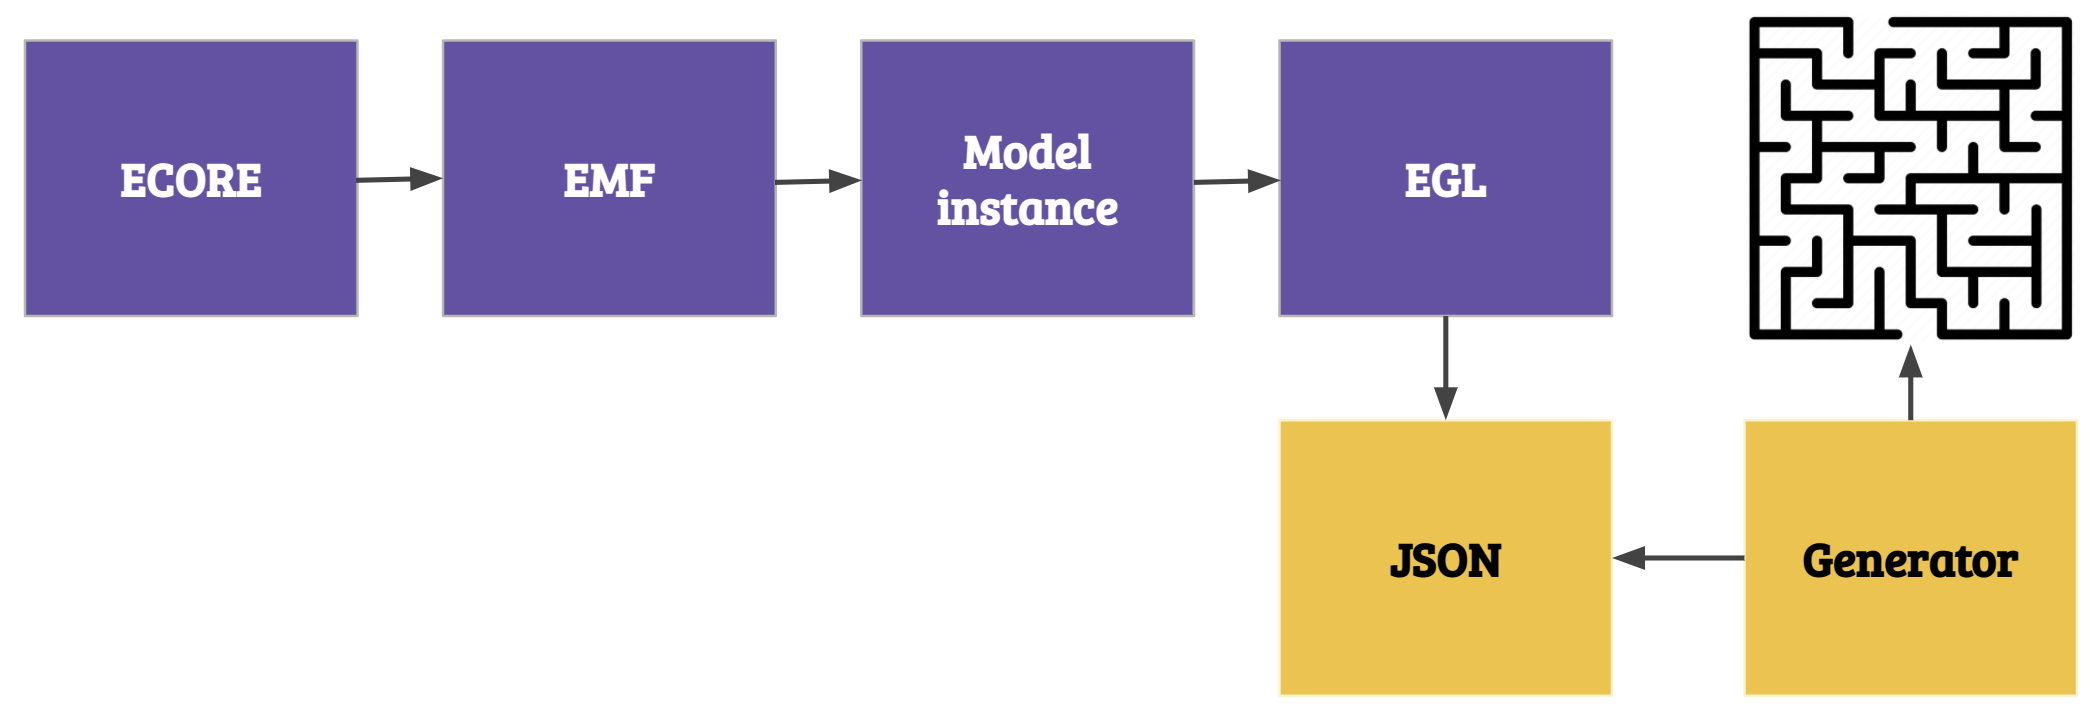
\includegraphics[width=\linewidth]{overview.png}
	\caption{Pipeline of the project}
	\label{fig:overview}
\end{figure}

\subsection{DSL}
The domain specific language represent the parameters used to generate the maze. Presented as a visual syntax in Figure \ref{fig:model}, it contains four types of generator. From left to right, generators are represented as blue rectangles: (1) \textit{RGen} is the first step of the maze generation, it gives the initial borders of the maze using a row count (\textit{RC}) and a column count (\textit{CC}) represented as red squares. (2) \textit{FPGen} inject maze cells in this initial shape to force a pattern, it allows users to create drawing in the maze. Forced cells are represented as orangish squares (\textit{Marked 15 with a CP}) where a point is defined inside of it. In Figure \ref{fig:model}, we only force a single cell. (3) \textit{SPGen} is the generation of a solution path with specific parameters, allowing to gives different behaviours from the general maze body. Used rates are represented as green circles. (4) \textit{MBGen} is the last step, the maze body generation. Using rates as green circles also. The main reason for choosing the visual, rather than textual, approach for the DSL  is for the representation of forced pattern cells in the maze where user is able to create more complex drawing. Based on Eugenia documentation\cite{noauthor_eugenia_nodate}, there is a way to integrate custom images into a DSL, after many hours of debugging, I was not able to do it, concluding this is probably a tool issue. My original idea was to integrate maze cells as in Figure \ref{fig:cells}.

\begin{figure}
	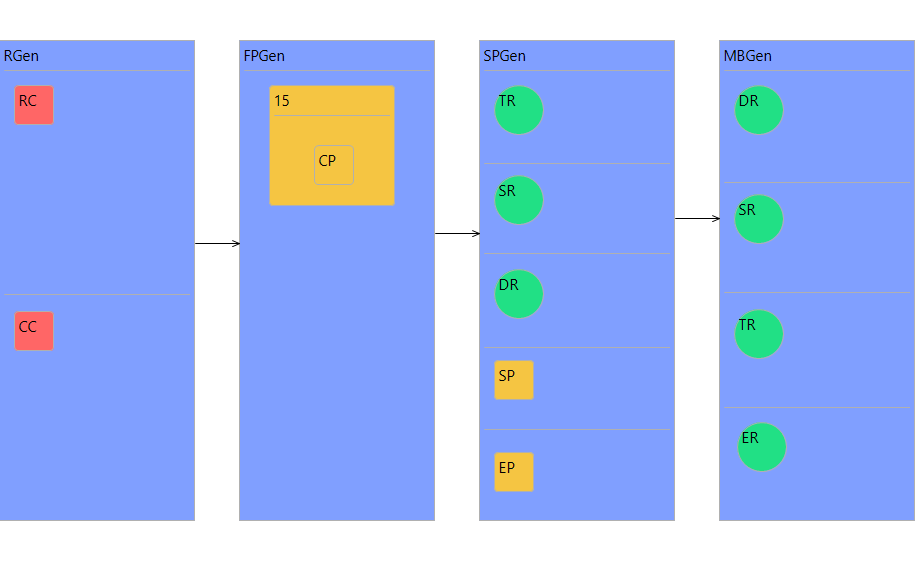
\includegraphics[width=\linewidth]{model.png}
	\caption{A model instance from the DSL}
	\label{fig:model}
\end{figure}

\paragraph{Types of rate}
Rates are represented as weights. Each cell types are associated with a rate category. These weights will be used to define how much theses associated cells will be present in the maze. The higher weight value is, the more the associated cell with be in the maze. DSL uses 4 types of rates: (1) StraightRate marked as \textit{SR} that represent weight of straight path. (2) TurnRate marked as \textit{TR} that represent uni-directional turning path. (3) DecisionRate marked as \textit{DR} that represent bi-directional turns and crossroads. This rate allow user to make the maze more complex to solve. (4) EndRate marked as \textit{ER} that represent the famous dead-end, also known as  \textit{cul-de-sac}. Weight are used in a probabilist approach. More details on this process will be given in the Generator section.

\begin{figure}
	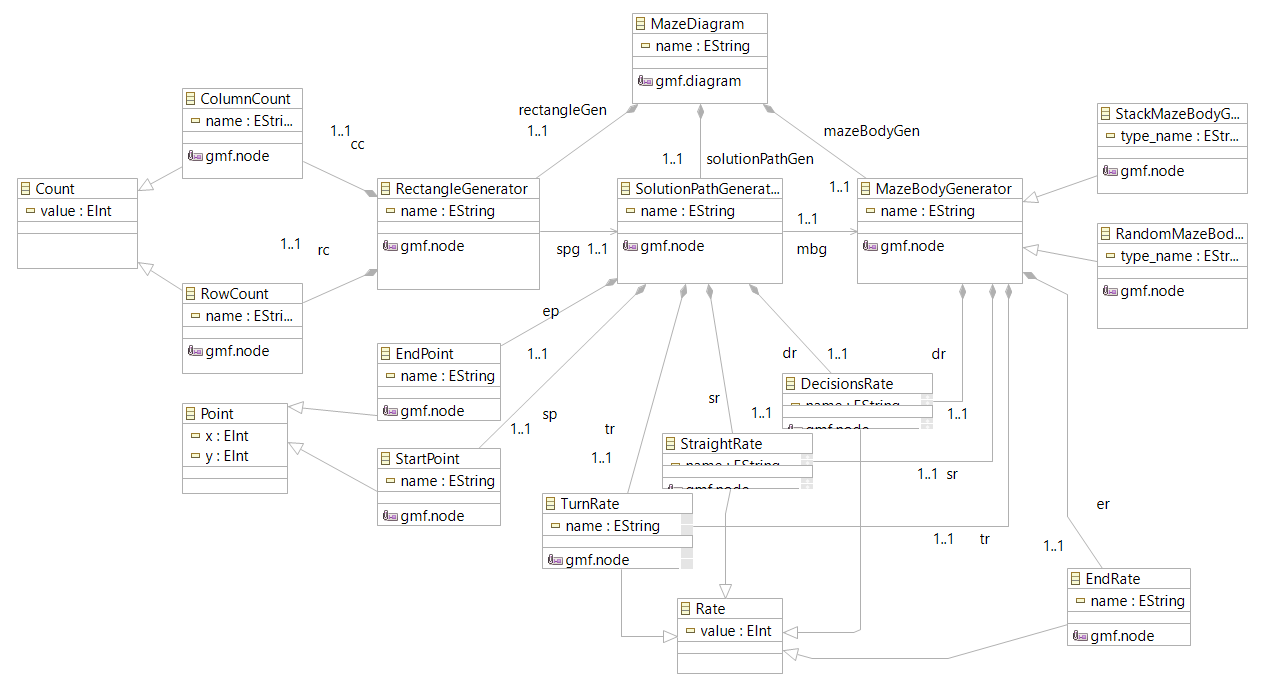
\includegraphics[width=\linewidth]{metamodel.png}
	\caption{Meta-model of the DSL}
	\label{fig:metamodel}
\end{figure}

\subsubsection{Meta-model}
As mentioned earlier, our DSL is a representation of different parameter types to generate a maze. Meta-model is refereed in Figure \ref{fig:metamodel}. This generation is a sequential order of four steps: rectangle, forced patterns, solution path, maze body. The root Class of the meta-model is \textit{MazeDiagram} with mandatory attributes to the four generators. Three abstract Class are used here to encapsulated shared concepts between generators: (1) \textit{Count} with a integer attribute \textit{value} used by \textit{RectangleGenerator} to represent row and column count. (2) \textit{Point} used to locate forced maze cells on the grid for \textit{ForcePatternGenerator} and also to locate starting and ending point for \textit{SolutionPathGenerator} (3) \textit{Rate} to give weigh values used by probabilistic algorithms that defines the solution path and the maze body (\textit{SolutionPathGenerator, MazeBodyGenerator}). Note the EndRate is only used during the maze body generation as it doesn't makes sense to create solution path with no possible exit. The use of multiplicity \textit{1..1} almost everywhere made sure every parameters are contained in the graph, so nothing will be missing during the generation. Multiplicity for \textit{mazeCells} is \textit{0..*} since forcing cells into the maze is an optional features. The attributes 'name' in each class are read-only with a default value. This field is important for the model transformation process.

\subsubsection{Model to Text Transformation }
Using a valid model instance, we can produce a JSON file that is readable by the Generator. Once this file is produced using an EGL defined transformation, the JSON is put into a folder where the Generator fetch data. No manual operations on the outputted file is needed. The 'name' attribute is used as keys in the JSON file, providing a perfect bridge of communication between the MDE and Software part of the project.

\subsection{Generator}
Build as an external object oriented program in Python. As presented in the Figure \ref{fig:class_diagram}, the software hold four main parts: (1) \textit{Cell feeding services} used to provide cell instances during the generation process that are valid considering neighbours and rate type choice. \textit{AllowCellTypeFeeder} provides possible cells concerning the neighbours cells, \textit{CellRateTypeFeeder} gives set of cell that are of a given rate type (2) \textit{Cell} is the internal representation of Maze cells in the program. \textit{Cell} class contains information that are not subject to changes during the generation and \textit{CellInfo} contains changeable informations. (3) \textit{Printing services} charged to gives readable output for the user. (4) \textit{Generation algorithms or the MazeGrid Class} for every ordered phase of the generation as represented in the DSL.

\begin{figure}
	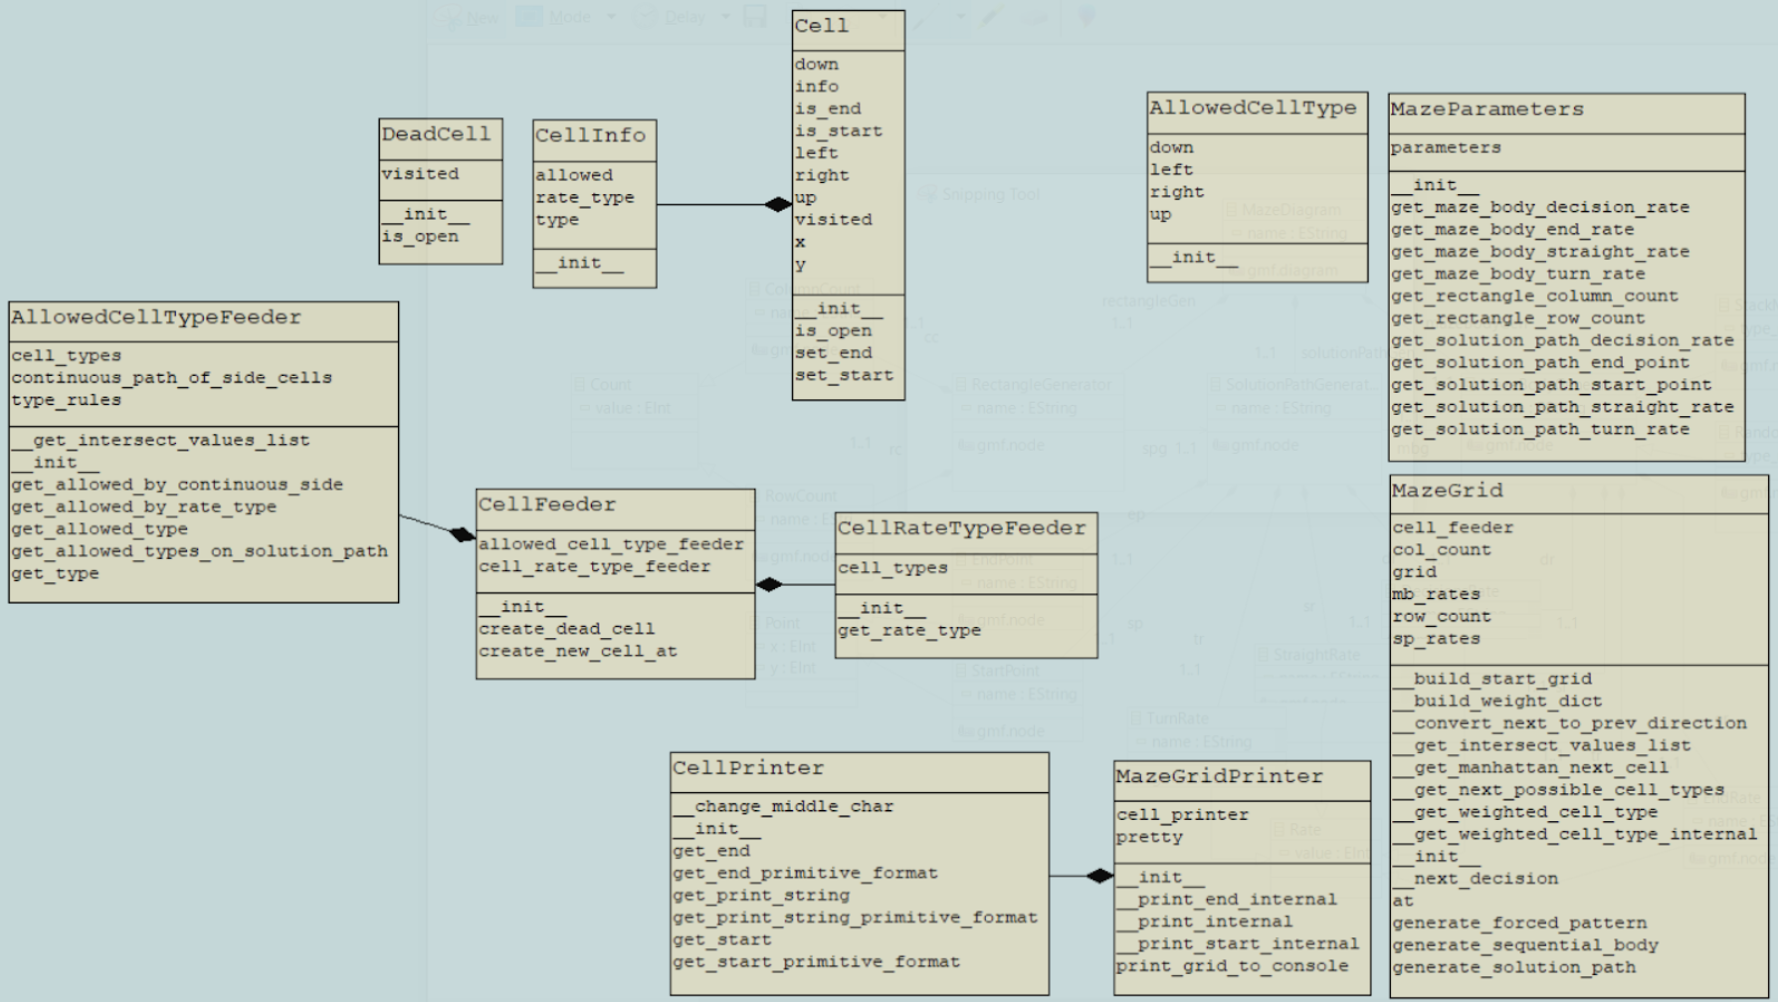
\includegraphics[width=\linewidth]{class_diagram.png}
	\caption{Class Diagram of the Python program}
	\label{fig:class_diagram}
\end{figure}

\subsubsection{Determining next generated cell}
There are five distinct parts to determine what will be the next generated cell in the maze. This process is roughly exposed in Figure \ref{fig:next_decision} and used for the solution path and the maze body generation steps, the steps are as follow: (1) Generate a list of possible cell types for the currently generated cell considering left, top, right, bottom neighbours (2) Use associated rate weights in the input JSON file to probabilistically determine what will be the next rate. (3) With this rate, generate a list of valid cell types (4) Intersect both list (5) Choose a random value within this list and assign the type to the currently generated cell.

\begin{figure}
	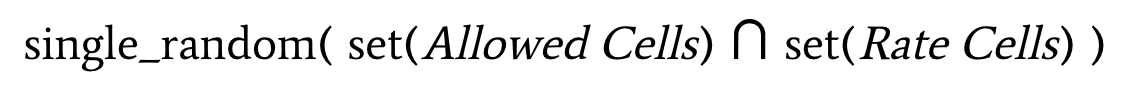
\includegraphics[width=\linewidth]{next_decision_formula.png}
	\caption{Formula for the next cell generation}
	\label{fig:next_decision}
\end{figure}

\subsubsection{Maze cells}
The generator uses a total of 16 maze cells types, as in Figure \ref{fig:cells}. Each cells have a list allowed neighbours, this list is computed in class \textit{AllowedCellTypeFeeder}. Generation algorithms will used this features to intersect will other desired cells types to make sure all cells can connect together at the end of the generation as mentioned earlier. Each cells have associated rate to it, the class \textit{CellRateTypeFeeder} is meant to build those lists.

\begin{figure}
	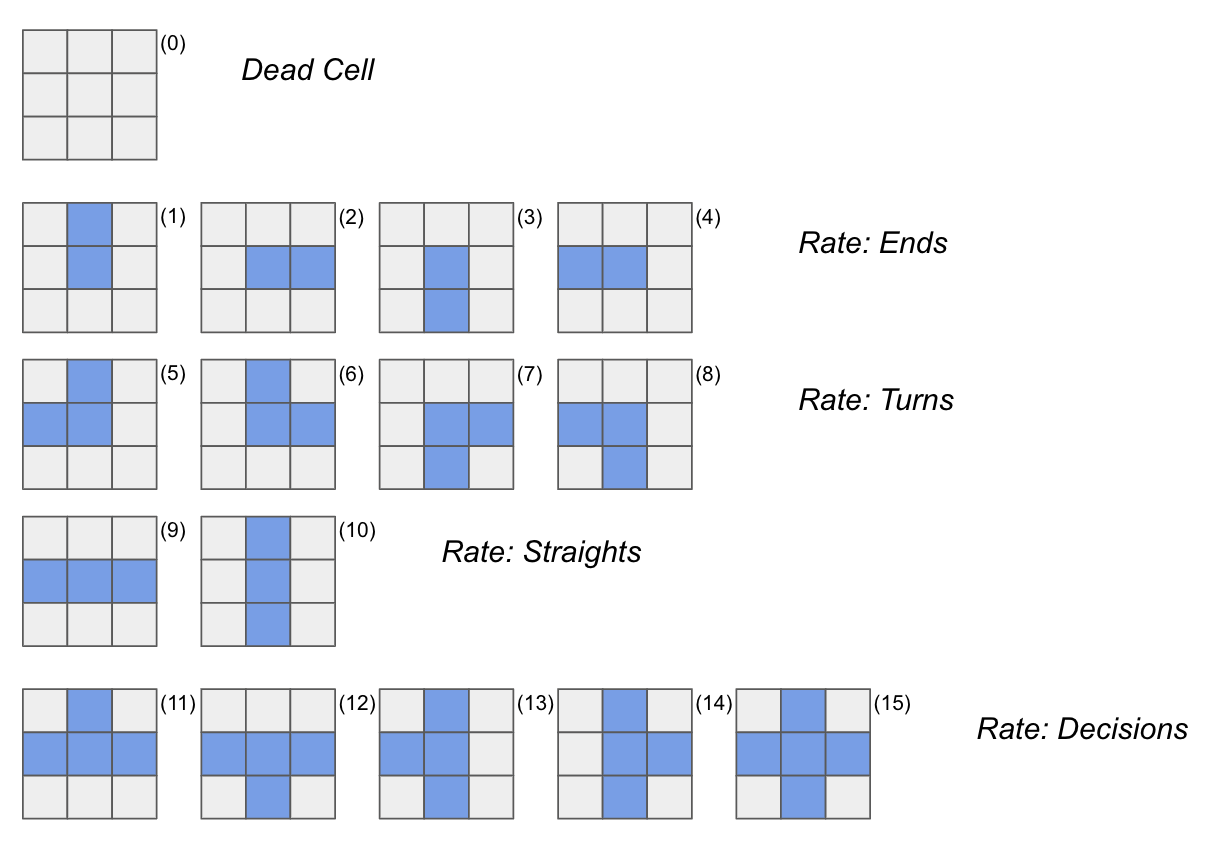
\includegraphics[width=\linewidth]{maze_cells_clean.png}
	\caption{Maze cells with associated rate type}
	\label{fig:cells}
\end{figure}

\begin{figure}
	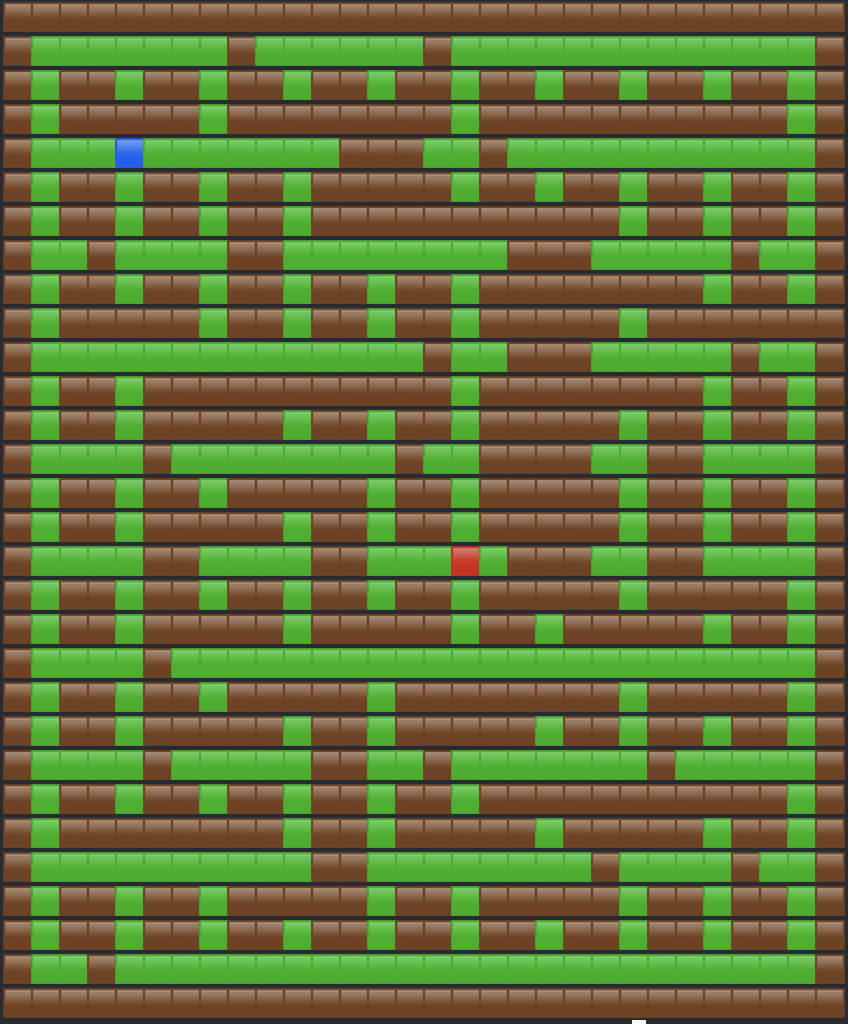
\includegraphics[width=\linewidth]{pretty_output.png}
	\caption{Maze output example}
	\label{fig:pretty_output}
\end{figure}

\subsubsection{Produced output}
The output is produced on the user console where the Python program got executed. Figure \ref{fig:pretty_output} illustrate this output. Tiles are to be considered as follow: (1) \textit{Brown} are the walls, (2) \textit{Green} are the paths, (4) Blue is the player spawn point and (4) \textit{Red} is the target point the player wants to reach.

\section{Evaluation}
The interesting part of this project is the MDE part since this is the real gain. Maze generation algorithm is nothing new in the world on computer science, this parameter-driven approach allow the justification of a DSL. This tool, with more work, could be used as an academic tool to learn about maze and the theory behind it, for example, we could try to find optimal parameters to output the most complex maze, or the easiest. We could also find how many decision a player as to do for finding the exit before considering the maze is not doable by a human being.

\begin{figure}
	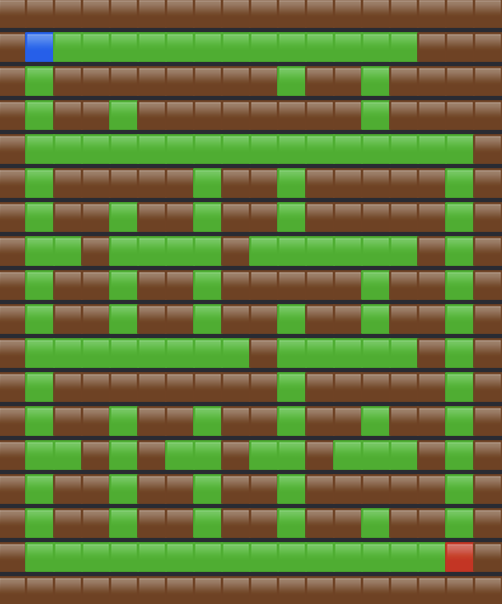
\includegraphics[width=50mm]{maze_diff.png}
	\centering
	\caption{Small maze with very different solution path rates and maze body rates}
	\label{fig:maze_diff}
\end{figure}

\begin{figure}
	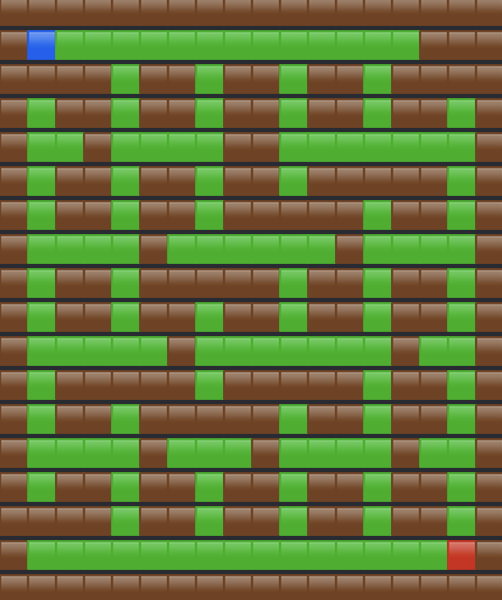
\includegraphics[width=50mm]{maze_dr.png}
	\centering
	\caption{Small maze with very high level of decision}
	\label{fig:maze_dr}
\end{figure}

\begin{figure}
	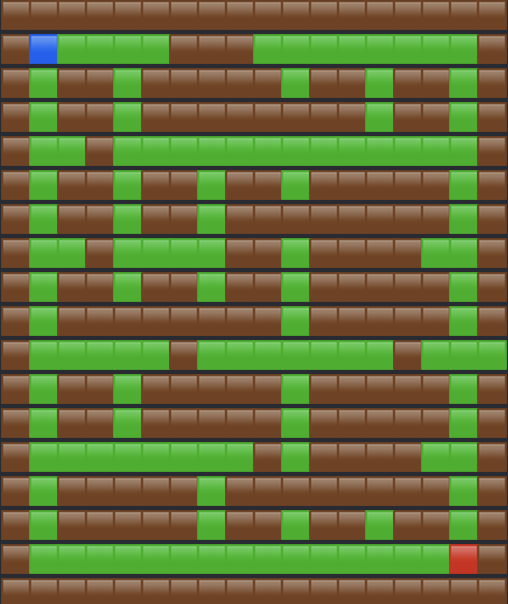
\includegraphics[width=50mm]{maze_draw.png}
	\centering
	\caption{Small maze with cross drawn in it}
	\label{fig:maze_draw}
\end{figure}

\section{Related Work}
As mentioned earlier, maze generation is not a new things. Plenty on online tools are available, sometimes with less parameters\cite{noauthor_maze_nodate}. Also, plenty of techniques exist, for example Kruskals’ algorithm ``can be used to splits the graph nodes into separate components and repeatedly unifies them using graph links\cite{bouda_day_2017}.'' Since the MDE community is very small today, I asked myself the question if a DSL to help for the generation of mazes exist already. It seems is doesn't in the case of a Maze and exist for a similar concept, a Pacman DSL\cite{leroy_create_nodate}. Their approach is a Executable DSL where models reacts to their environment allowing simulation of the Pacman game.

\section{Conclusion}
The goal of giving a more user-friendly orientation to generate maze is a success within my work, except for the maze cell design representation in the DSL. The Generator program is also capable to give distinct behaviour to the solution path and the maze body, giving personalities to mazes. As shown in  \ref{fig:maze_diff}, we can clearly identify the solution as composed essentially with straight cells and the maze body with decision cells. In terms of implementation, it lacks in the generation of a single solution, especially in small mazes when we apply a high decision rate we end up having too much possible ways to reach the finish point, as shown in Figure \ref{fig:maze_diff}. This problem could have been solved with the implementation of a maze body generation algorithm based on a \textit{stack structure} where every cells in it represent an open decision on the solution path from where generation would be triggered. The force pattern feature is a success as it able user to create drawing in the maze, as shown in Figure  \ref{fig:maze_draw}. Some problematic encountered was the creation executing \textit{EVL} constants. With the current implementation a user could, for example, define a player spawn point outside of the actual maze borders, creating a exception to be thrown in the Generator program. This makes the DSL lack in terms of robustness.

\bibliography{mybibfile}

\end{document}